\chapter{Bài 7. Gia tốc - Chuyển động thẳng biến đổi đều }
\begin{center}
\itshape (4 tiết)
\end{center}
\section{MỤC TIÊU DẠY HỌC}
\begin{center}
	\begin{longtable}{|M{2.5cm}|L{12.5cm}|M{2cm}|}
		\hline
		\thead{Biểu hiện\\ năng lực} & \thead{Mục tiêu} & \thead{STT}\\
		\hline
		\multicolumn{3}{|c|}{\textbf{ Năng lực vật lí}}\\
		\hline
		1.1 & Lập luận dựa vào sự biến đổi vận tốc trong chuyển động thẳng, rút ra được công thức tính gia tốc.  & 1\\
		\hline
		1.1 & Nêu được ý nghĩa, đơn vị của gia tốc.  & 2\\
		\hline
		1.2 & Dựa trên số liệu cho trước vẽ được đồ thị vận tốc – thời gian trong chuyển động thẳng. & 3\\
		\hline
		1.2 & Vận dụng đồ thị vận tốc – thời gian để tính được độ dịch chuyển và gia tốc trong một số trường hợp đơn giản. & 4\\
		\hline
		1.2 & Rút ra được các công thức của chuyển động thẳng biến đổi đều (không được dùng tích phân). & 5\\
		\hline
		1.2 & Vận dụng được các công thức của chuyển động thẳng biến đổi đều. & 6\\
		\hline
		\multicolumn{3}{|c|}{\textbf{Năng lực chung}}\\
		\hline
		GT - HT & Chủ động trong giao tiếp khi làm việc nhóm; biết khiêm tốn tiếp thu sự góp ý và nhiệt tình chia sẻ, hỗ trợ các thành viên trong nhóm. & 7\\
		\hline
		TC - TH & Chủ động, tích cực thực hiện các nhiệm vụ được đặt ra cho các nhóm; tự điều chỉnh thái độ, hành vi của bản thân, bình tĩnh và có cách cư xử đúng khi giao tiếp trong quá trình làm việc nhóm. & 8\\
		\hline
	\end{longtable}
\end{center}
\section{THIẾT BỊ DẠY HỌC VÀ HỌC LIỆU}
\begin{itemize}
	\item Tivi/máy chiếu.
	\item Phiếu thảo luận nhóm.
\end{itemize}
\section{TIẾN TRÌNH DẠY HỌC}
\subsection{TIẾN TRÌNH}
\begin{center}
	\begin{longtable}{|L{2.75cm}|C{1.25cm}|L{5cm}|L{3.5cm}|L{4cm}|}
		\hline
		\thead{Tiến trình} & \thead{Mục\\tiêu} & \thead{Nội dung dạy học \\trọng tâm} & \thead{PP,\\ KTDH} & \thead{Phương pháp \\đánh giá}\\
		\hline
		\textbf{Hoạt động 1:} Tìm hiểu khái niệm và ý nghĩa của gia tốc. & 1, 2, 7, 8 & Công thức tính gia tốc, ý nghĩa và đơn vị của gia tốc.&PP: Dạy học giải quyết vấn đề, thuyết trình. & GV đánh giá dựa trên kết quả báo cáo thảo luận nhóm của HS.\newline
		PP đánh giá: quan sát, nghe.\\
		\hline
		\textbf{Hoạt động 2:} Vận dụng đồ thị vận tốc – thời gian để tính độ dịch chuyển và gia tốc. & 3, 4, 7, 8 & Đồ thị vận tốc – thời gian trong chuyển động thẳng biến đổi đều.\newline
		Vận dụng đồ thị vận tốc – thời gian để tính độ dịch chuyển và gia tốc trong trường hợp đơn giản.
		& PP dạy học: Dạy học hợp tác, thuyết trình.\newline
		KTDH: Chia sẻ cặp đôi.
		& GV đánh giá dựa trên kết quả trên phiếu học tập và bài báo cáo của nhóm HS.\newline
		PP đánh giá: quan sát, nghe.\\
		\hline
		\textbf{Hoạt động 3:} Rút ra các công thức của chuyển động thẳng biến đổi đều. & 5, 7, 8 & Các công thức chuyển động thẳng biến đổi đều. & PP: Dạy học hợp tác. & GV đánh giá dựa trên kết quả hoạt động nhóm của HS trên phiếu học tập.\newline
		PP đánh giá: quan sát, nghe.\\
		\hline
		\textbf{Hoạt động 4:} Luyện tập. & 3, 4, 6 & Vận dụng các công thức chuyển động thẳng biến đổi đều. & PP: Đàm thoại & GV đánh giá dựa trên bài tập cá nhân của HS.\newline
		PP đánh giá: quan sát.\\
		\hline
	\end{longtable}
\end{center}
\subsection{CÁC HOẠT ĐỘNG HỌC}
\hoatdong{
Tìm hiểu khái niệm và ý nghĩa của gia tốc
}
{HS rút ra được công thức tính gia tốc.
	
HS nêu được ý nghĩa và đơn vị của gia tốc.
}
{
Phiếu hoạt động nhóm số 1 + Phần trình bày của nhóm HS.
}
{
\textit{\underline{* GV chuyển giao nhiệm vụ học tập}}\\
GV chia lớp thành 4 nhóm. GV yêu cầu HS đọc kĩ nhiệm vụ của hoạt động 1 và thảo luận theo nhóm đã chia. Sau 10 phút, GV gọi 1 nhóm lên trình bày kết quả thảo luận của nhóm, các nhóm còn lại góp ý/bổ sung.\\
\textit{\underline{* HS thực hiện nhiệm vụ học tập}}\\
HS \textit{(làm việc theo nhóm)}: Tiến hành thảo luận, đưa ra đáp án + lời giải thích cho mỗi tình huống trong phiếu học tập số 1. Nhóm HS trình bày kết quả vào phiếu học tập và thống nhất chọn đại diện báo cáo.\\
GV: Theo dõi các nhóm thảo luận để phát hiện kịp thời vấn đề mà nhóm HS gặp phải, từ đó đưa ra sự định hướng, hỗ trợ phù hợp cho mỗi nhóm.\\
\textit{\underline{* HS báo cáo kết quả thực hiện nhiệm vụ học tập}}\\
GV: Yêu cầu đại diện của 1 nhóm HS lên trình bày kết quả hoạt động 1. Các nhóm còn lại chú ý theo dõi để nhận xét.

HS: Đặt câu hỏi, góp ý.

GV: Chỉnh lí, hợp thức hoá kiến thức.

GV: Từ kết quả báo cáo của HS, GV giới thiệu khái niệm và ý nghĩa của gia tốc.

HS: Ghi chép nội dung trọng tâm vào vở.
}
%%%%%%%%%%%%%%%%%%%%%%%%%%%%%%%%%%%%%%%%%%%%%%%%%%%%%%%%%%%%%%%
\hoatdong{
Vận dụng đồ thị vận tốc – thời gian để tính độ dịch chuyển và gia tốc
}
{
	HS vận dụng đồ thị vận tốc – thời gian để tính được độ dịch chuyển và gia tốc trong một số trường hợp đơn giản.
}
{
Phiếu hoạt động nhóm số 2 + Phần trình bày của HS.
}
{
\textit{\underline{GV chuyển giao nhiệm vụ học tập}}\\
GV hướng dẫn HS cách xác định độ dịch chuyển từ đồ thị vận tốc – thời gian.

GV chia lớp thành các nhóm đôi. Một nửa số nhóm thực hiện câu a, các nhóm còn lại thực hiện câu b. 

GV yêu cầu HS đọc kĩ nhiệm vụ của hoạt động 2 và thảo luận theo nhóm đã chia. Sau 10 phút, GV gọi 2 HS đại diện của 2 nhóm lên trình bày kết quả hoạt động, các nhóm còn lại góp ý/bổ sung.\\
\textit{\underline{HS thực hiện nhiệm vụ học tập}}\\
HS \textit{(làm việc theo nhóm đôi)}: Tiến hành thảo luận, đưa ra đáp án trong phiếu học tập số 2. 

GV: Theo dõi để phát hiện các HS gặp khó khăn, từ đó đưa ra sự định hướng, hỗ trợ phù hợp cho mỗi HS.\\
\textit{\underline{HS báo cáo kết quả thực hiện nhiệm vụ học tập}}\\
GV: Yêu cầu đại diện của 2 nhóm HS lên trình bày kết quả hoạt động 2. Các nhóm còn lại chú ý theo dõi để nhận xét.

HS: Đặt câu hỏi, góp ý.

GV: Chỉnh lí, hợp thức hoá kiến thức.


}
%%%%%%%%%%%%%%%%%%%%%%%%%%%%%%%%%%%%%%%%%%%%%%%%%%%%%%%%%%%
\hoatdong{
Rút ra các công thức của chuyển động thẳng biến đổi đều.
}
{
HS vận dụng đồ thị vận tốc – thời gian để rút ra công thức tính độ dịch chuyển trong chuyển động thẳng biến đổi đều.
}
{
	Phiếu hoạt động nhóm số 3 + Phần trình bày của HS.
}
{
\textit{\underline{* GV chuyển giao nhiệm vụ học tập}}\\
GV yêu cầu HS hoạt động theo nhóm lớn đã chia và đọc kĩ nhiệm vụ của hoạt động 3. Sau 10 phút, GV gọi 1 HS đại diện của 1 nhóm lên trình bày kết quả hoạt động, các nhóm còn lại góp ý/bổ sung.\\
\textit{\underline{* HS thực hiện nhiệm vụ học tập}}
HS (làm việc theo nhóm lớn): Tiến hành thảo luận, đưa ra đáp án trong phiếu học tập số 3. 

GV: Theo dõi để phát hiện các HS gặp khó khăn, từ đó đưa ra sự định hướng, hỗ trợ phù hợp cho mỗi HS.\\
\textit{\underline{* HS báo cáo kết quả thực hiện nhiệm vụ học tập}}\\
GV: Yêu cầu đại diện của 1 nhóm HS lên trình bày kết quả hoạt động 3. Các nhóm còn lại chú ý theo dõi để nhận xét.

HS: Đặt câu hỏi, góp ý.

GV: Chỉnh lí, hợp thức hoá kiến thức.
}
%%%%%%%%%%%%%%%%%%%%%%%%%%%%%%%%%%%%%%%%%%%%%
\hoatdong{
Luyện tập.
}
{
HS vận dụng được các công thức của chuyển động thẳng biến đổi đều.
}
{
Bài tập cá nhân của học sinh.
}
{
\textit{\underline{GV chuyển giao nhiệm vụ học tập}}\\
GV lần lượt chuyển giao từng bài tập, yêu cầu HS hoạt động cá nhân để giải.\\
\textit{\underline{HS thực hiện nhiệm vụ học tập}}\\
HS \textit{(làm việc cá nhân)}:  Giải bài tập trong phiếu bài tập được GV giao. 

GV: Theo dõi để phát hiện các HS gặp khó khăn, từ đó đưa ra sự định hướng, hỗ trợ phù hợp cho mỗi HS.\\
\textit{\underline{HS báo cáo kết quả thực hiện nhiệm vụ học tập}}\\
GV: Mời HS lên bảng giải bài tập.

HS: Đặt câu hỏi, góp ý.

GV: Chỉnh lí, hợp thức hoá kiến thức.
}

\section{HỒ SƠ DẠY HỌC}
\subsection{NỘI DUNG DẠY HỌC}
\begin{enumerate}[label=\bfseries\arabic*.]
	\item \textbf{Gia tốc}\\
	Gia tốc là đại lượng đặc trưng cho độ biến thiên của vận tốc theo thời gian. Trong chuyển động thẳng, gia tốc trung bình được xác định theo biểu thức:
	\begin{equation}
		a_{tb}=\dfrac{\Delta v}{\Delta t}=\dfrac{v-v_0}{\Delta t}
	\end{equation}
	Trong hệ SI, đơn vị của gia tốc là $\si{\meter/\second^2}$.\\
	Khi $\Delta t$ rất nhỏ, gia tốc trung bình trở thành gia tốc tức thời. Gia tốc tức thời tại một thời điểm có giá trị bằng độ dốc của tiếp tuyến của đồ thị vận tốc – thời gian.\\
	Dựa vào gia tốc tức thời, ta có thể phân chuyển động thẳng thành 3 loại:
	\begin{center}
		\begin{tabular}{|M{5cm}|M{5cm}|M{6cm}|}
			\hline
			Chuyển động thẳng đều & Chuyển động thẳng biến đổi đều & Chuyển động thẳng biến đổi phức tạp\\
			\hline
			$a=0$ & $a=const\neq0$ & $a\neq0$ nhưng không phải hằng số\\
			\hline
		\end{tabular}
	\end{center}
	\item \textbf{Đồ thị vận tốc - thời gian}\\
	\begin{enumerate}[label=\bfseries \itshape 2.\arabic*., nolistsep]
		\item  \textbf{\textit{Đồ thị vận tốc – thời gian của chuyển động thẳng biến đổi đều}}\\
		Chuyển động thẳng biến đổi đều là chuyển động thẳng mà vận tốc có độ lớn tăng đều hoặc giảm đều theo thời gian:
		\begin{itemize}
			\item chuyển động thẳng có độ lớn vận tốc tăng đều theo thời gian gọi là chuyển động thẳng nhanh dần đều ( $\vec{a}\uparrow\uparrow\vec{v}$ hay $a\cdot v>0$);
			\item chuyển động thẳng có độ lớn vận tốc giảm dần theo thời gian gọi là chuyển động thẳng chậm dần đều ($\vec{a}\uparrow\downarrow\vec{v}$  hay  $a\cdot v<0$).
			
		\end{itemize}
		Nếu tại thời điểm $t_0=0$   vật có vận tốc $v_0$ thì phương trình vận tốc của vật tại thời điểm $t$:
		\begin{equation}
			v=v_0+at
		\end{equation}
		Đồ thị vận tốc – thời gian của vật chuyển động thẳng biến đổi đều có dạng:
		\begin{center}
			\begin{tabular}{M{8.5cm}M{8.5cm}}
				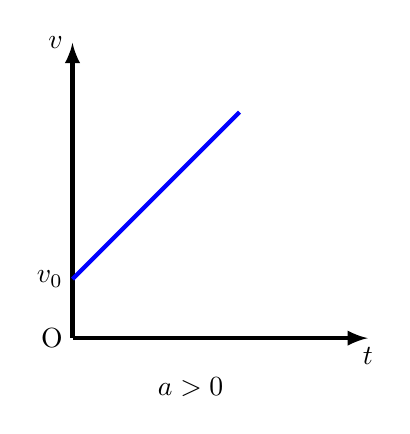
\begin{tikzpicture}[scale=0.75]  
					\coordinate (O) at(0,0);
					\coordinate (x) at(5,0);
					\coordinate (y) at(0,5);
					\coordinate (v0) at(0,1);
					\draw[-latex, line width=1.5pt] (O)--(x);
					\draw[-latex, line width=1.5pt] (O)--(y);
					\draw[blue, line width=1.5pt] (v0)--+(45:4);
					\node[below] at(x) {$t$};
					\node[left] at(y) {$v$};
					\node[left] at(v0) {$v_0$};
					\node[left] at(O) {O};
					\node[below] at (2,-0.5) {$a>0$};
				\end{tikzpicture}
				&
				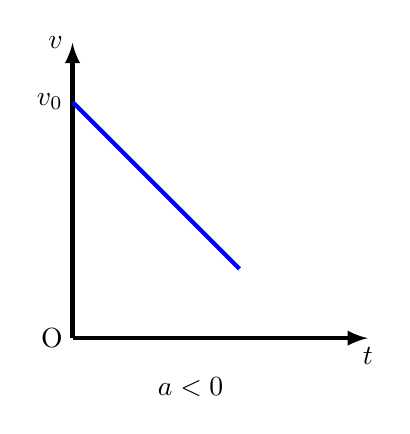
\begin{tikzpicture}  [scale=0.75] 
					\coordinate (O) at(0,0);
					\coordinate (x) at(5,0);
					\coordinate (y) at(0,5);
					\coordinate (v0) at(0,4);
					\draw[-latex, line width=1.5pt] (O)--(x);
					\draw[-latex, line width=1.5pt] (O)--(y);
					\draw[blue, line width=1.5pt] (v0)--+(-45:4);
					\node[below] at(x) {$t$};
					\node[left] at(y) {$v$};
					\node[left] at(v0) {$v_0$};
					\node[left] at(O) {O};
					\node[below] at (2,-0.5) {$a<0$};
				\end{tikzpicture}
			\end{tabular}
		\end{center}
		\item \textbf{\textit{Vận dụng độ thị vận tốc – thời gian để tính độ dịch chuyển}}\\
		\begin{center}
			\begin{tabular}{M{8cm}M{8cm}}
				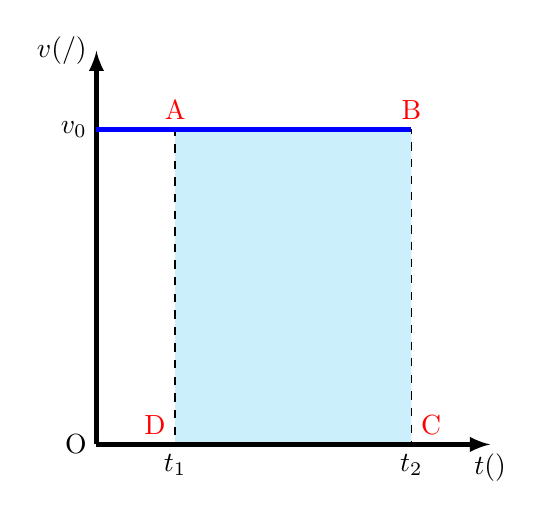
\begin{tikzpicture}  
					\coordinate (O) at(0,0);
					\coordinate (x) at(5,0);
					\coordinate (y) at(0,5);
					\coordinate (v0) at(0,4);
					\coordinate (A) at(1,4);
					\coordinate (B) at(4,4);
					\coordinate (C) at(4,0);
					\coordinate (D) at(1,0);
					\draw[-latex, line width=1.5pt] (O)--(y);
					\fill[cyan, opacity=0.2] (A)--(B)--(C)--(D)--(A);
					\draw[line width=0.5pt,black, dashed] (A)--(B)--(C)--(D)--(A);
					\draw[-latex, line width=1.5pt] (O)--(x);
					\draw[blue, line width=1.5pt] (v0)--(B);
					\node[below] at(x) {$\xsi{t}{\left(\second\right)}$};
					\node[left] at(y) {$\xsi{v}{(\meter/\second)}$};
					\node[left] at(v0) {$v_0$};
					\node[left] at(O) {O};
					\node[below] at (C) {$t_2$};
					\node[below] at (D) {$t_1$};
					\node[above, red] at(A) {A};
					\node[above, red] at(B) {B};
					\node[above right, red] at(C) {C};
					\node[above left, red] at(D) {D};
				\end{tikzpicture}
				&
				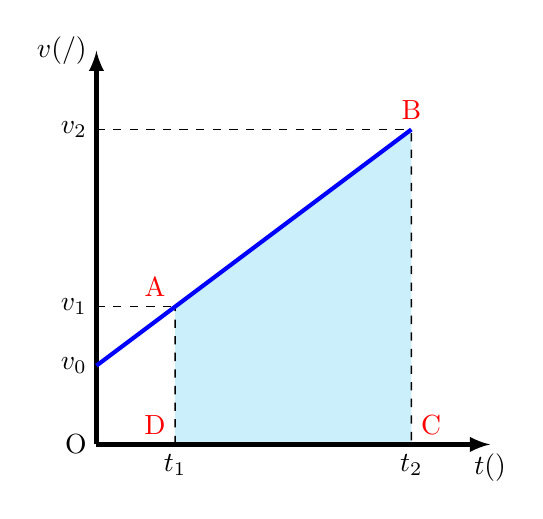
\begin{tikzpicture}  
					\coordinate (O) at(0,0);
					\coordinate (x) at(5,0);
					\coordinate (y) at(0,5);
					\coordinate (v0) at(0,1);
					\coordinate (v1) at(0,1.75);
					\coordinate (v2) at(0,4);
					\coordinate (B) at(4,4);
					\coordinate (A) at(1,1.75);
					\coordinate (C) at(4,0);
					\coordinate (D) at(1,0);
					\fill[cyan, opacity=0.2] (A)--(B)--(C)--(D)--(A);
					\draw[line width=0.5pt,black, dashed] (A)--(B)--(C)--(D)--(A);
					\draw[line width=0.5pt, dashed] (v1)--(A);
					\draw[line width=0.5pt, dashed] (v2)--(B);
					\draw[-latex, line width=1.5pt] (O)--(x);
					\draw[-latex, line width=1.5pt] (O)--(y);
					\draw[blue, line width=1.5pt] (v0)--(B);
					\node[below] at(x) {$\xsi{t}{\left(\second\right)}$};
					\node[left] at(y) {$\xsi{v}{(\meter/\second)}$};
					\node[left] at(v0) {$v_0$};
					\node[left] at(v1) {$v_1$};
					\node[left] at(0,4) {$v_2$};
					\node[left] at(O) {O};
					\node[below] at (C) {$t_2$};
					\node[below] at (D) {$t_1$};
					\node[above left, red] at(A) {A};
					\node[above, red] at(B) {B};
					\node[above right, red] at(C) {C};
					\node[above left, red] at(D) {D};
				\end{tikzpicture}\\
				Đồ thị $v-t$ trong chuyển động\newline thẳng đều. & Đồ thị $v-t$ trong chuyển động \newline thẳng biến đổi đều.
			\end{tabular}
		\end{center}
		Độ dịch chuyển của vật trong khoảng thời gian từ $t_1$ đến $t_2$ được xác định bằng phần diện tích giới hạn bởi các đường $v\left(t\right)$, $v=0$ , $t=t_1$, $t=t_2$  trong đồ thị $\left(v-t\right)$.
	\end{enumerate}
	\item \textbf{Các phương trình của chuyển động thẳng biến đổi đều}\\
	\begin{itemize}[topsep=0pt]
		\item Phương trình gia tốc: $a=const$;
		\item Phương trình vận tốc: $v=v_0+at$ với $v=v_0$ khi $t_0=0$;
		\item Phương trình quãng đường: $s=v_0t+\dfrac{1}{2}at^2$;
		\item Phương trình toạ độ: $x=x_0+v_0t+\dfrac{1}{2}at^2$;
		\item Phương trình độc lập thời gian:
		$v^2-v^2_0=2as$.
	\end{itemize}
\end{enumerate}
\subsection{CÁC  HỒ SƠ KHÁC}
Phiếu học tập\newpage
\textbf{* Phiếu số 1:} Tìm hiểu khái niệm và ý nghĩa của gia tốc.
\begin{center}
	\begin{longtable}{|L{8.5cm}L{8.5cm}|}
		\hline
		\multicolumn{2}{|c|}{\thead{PHIẾU HỌC TẬP SỐ 1 (NHÓM LỚN)\\	TÌM HIỂU KHÁI NIỆM VÀ Ý NGHĨA GIA TỐC
		}}\\
		\hline
		Lớp: \dotfill & Nhóm: \dotfill\\
		\multicolumn{2}{|l|}{Tên: \dotfill}\\
		\hline
		\multicolumn{2}{|L{17cm}|}{\textbf{Nhiệm vụ:} Trong mỗi tình huống sau đây, hãy chỉ ra đối tượng có khả năng tăng tốc hiệu quả hơn (khả năng tăng tốc nhanh hơn) và đưa ra lời giải thích cho lựa chọn của em?}\\
		\hline
		\multicolumn{2}{|c|}{\textbf{Tình huống 1}}\\
		\multicolumn{2}{|L{17cm}|}{
			\begin{itemize}[topsep=0pt]
				\item Báo guépard có khả năng tăng tốc từ $\SI{0}{\kilo\meter/\hour}$ lên $\SI{96}{\kilo\meter/\hour}$ trong thời gian $\SI{3}{\second}$.
				\item Xe đua F1 có khả năng tăng tốc từ $\SI{0}{\meter/\second}$  lên $\SI{25}{\meter/\second}$  trong khoảng thời gian $\SI{3}{\second}$.
			\end{itemize}	
			\begin{center}
				\begin{tabular}{M{6cm}M{2cm}M{6cm}}
						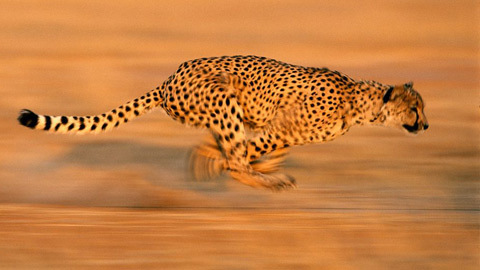
\includegraphics[scale=0.3]{figs/G10-BAI7-1}& & 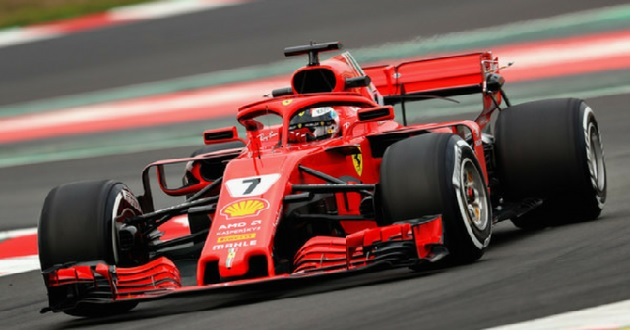
\includegraphics[scale=0.3]{figs/G10-BAI7-2}\\
						Báo guépard && Xe đua F1\\
				\end{tabular}
			\end{center}
			\dotfill
		}\\
		\multicolumn{2}{|L{17cm}|}{
			\dotfill
		}\\
		
		\multicolumn{2}{|L{17cm}|}{
			\dotfill
		}\\
		\hline
		\multicolumn{2}{|c|}{\textbf{Tình huống 2}}\\
		\multicolumn{2}{|L{17cm}|}{
			\begin{itemize}[topsep=0pt]
				\item Xe Porsche 911 Turbo S Lightweight 2021 có khả năng tăng tốc từ  $\SI{0}{\kilo\meter/\hour}$ lên $\SI{96}{\kilo\meter/\hour}$  trong thời gian $\SI{2.1}{\second}$.
				\item Xe Lamborghini Huracan Performante có khả năng tăng tốc từ $\SI{0}{\kilo\meter/\hour}$  lên $\SI{96}{\kilo\meter/\hour}$  trong thời gian $\SI{2.2}{\second}$.
			\end{itemize}	
			\begin{center}
				\begin{tabular}{M{6cm}M{2cm}M{6cm}}
					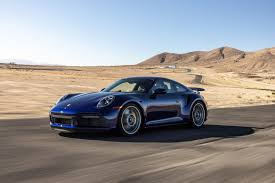
\includegraphics[scale=0.5]{figs/G10-BAI7-3}& & 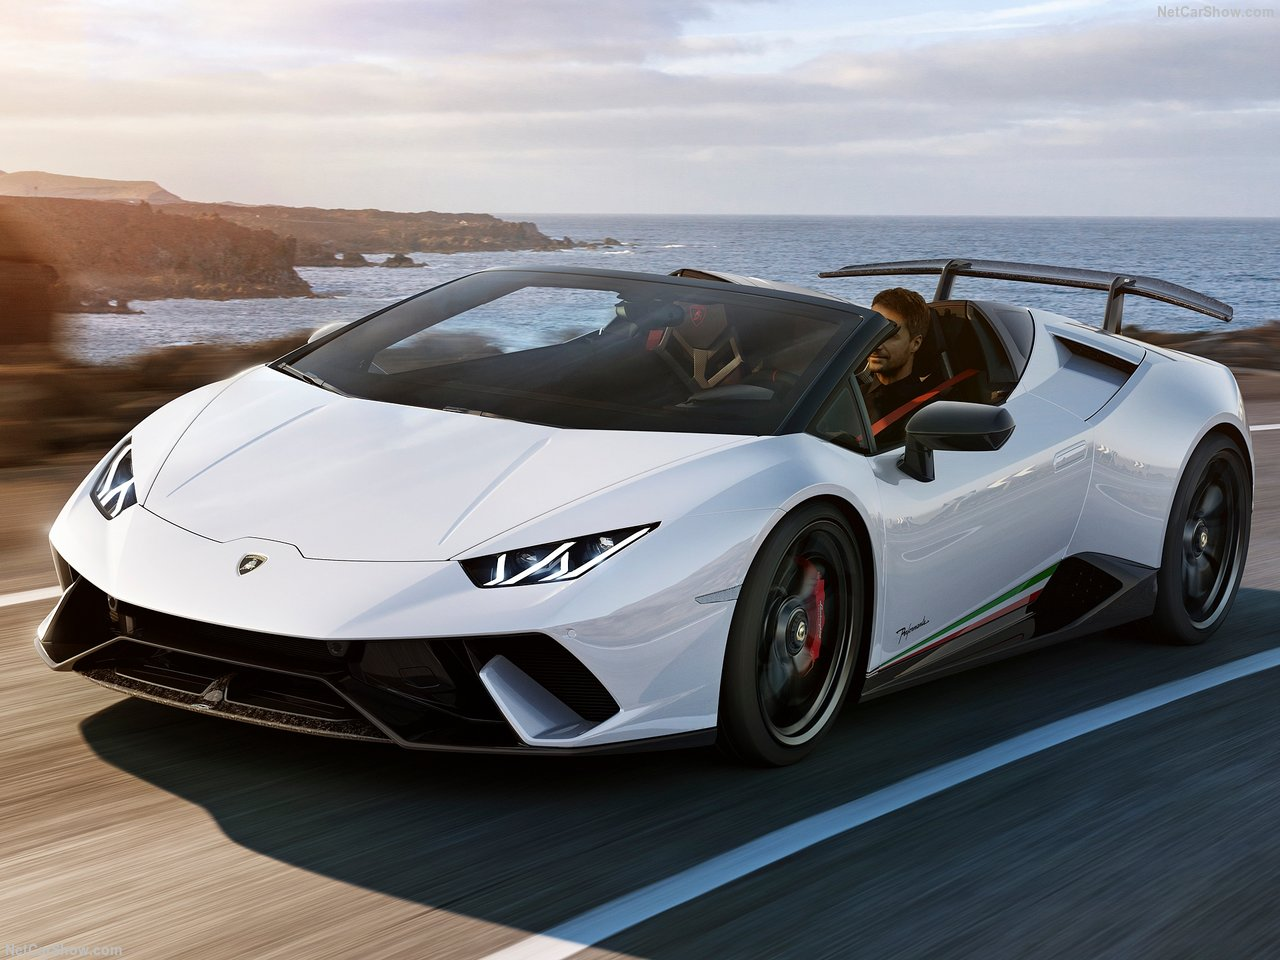
\includegraphics[scale=0.1]{figs/G10-BAI7-4}\\
					Xe Porsche 911 Turbo S Lightweight 2021 && Xe Lamborghini Huracan Performante\\
				\end{tabular}
			\end{center}
			\dotfill
		}\\
		\multicolumn{2}{|L{17cm}|}{
			\dotfill
		}\\
		
		\multicolumn{2}{|L{17cm}|}{
			\dotfill
		}\\
		\hline
		\multicolumn{2}{|c|}{\textbf{Tình huống 3}}\\
		\multicolumn{2}{|L{17cm}|}{
			\begin{itemize}[topsep=0pt]
				\item Vận động viên A từ khi xuất phát đến khi đạt tốc độ $\SI{9}{\meter/\second}$  mất thời gian $\SI{2}{\second}$.
				\item Vận động viên B từ khi xuất phát đến khi đạt tốc độ $\SI{6}{\meter/\second}$  mất thời gian $\SI{1.5}{\second}$.
			\end{itemize}	
			\dotfill
		}\\
		\multicolumn{2}{|L{17cm}|}{
			\dotfill
		}\\
		
		\multicolumn{2}{|L{17cm}|}{
			\dotfill
		}\\
		\multicolumn{2}{|L{17cm}|}{
			\dotfill
		}\\
		\hline
	\end{longtable}
\end{center}
\textbf{Phiếu số 2:} Vận dụng đồ thị $v-t$ để xác định độ dịch chuyển và gia tốc.
\begin{center}
	\begin{longtable}{|L{8.5cm}|L{8.5cm}|}
		\hline
		\multicolumn{2}{|M{17cm}|}{\bfseries PHIẾU HỌC TẬP SỐ 2 \textit{(NHÓM ĐÔI)}\newline
			VẬN DỤNG ĐỒ THỊ  ĐỂ XÁC ĐỊNH ĐỘ DỊCH CHUYỂN VÀ GIA TỐC
		}\\
		\hline
		\multicolumn{2}{|M{17cm}|}{Lớp: \dotfill}\\
		\multicolumn{2}{|M{17cm}|}{Nhóm: \dotfill}\\
		\multicolumn{2}{|M{17cm}|}{Tên: \dotfill}\\
		\hline
		\multicolumn{2}{|L{17cm}|}{
			\textbf{Nhiệm vụ:}	Dựa vào đồ thị $\left(v-t\right)$ của vật chuyển động trong hình, hãy xác định gia tốc và độ dịch chuyển của vật trong các giai đoạn:
			\begin{center}
				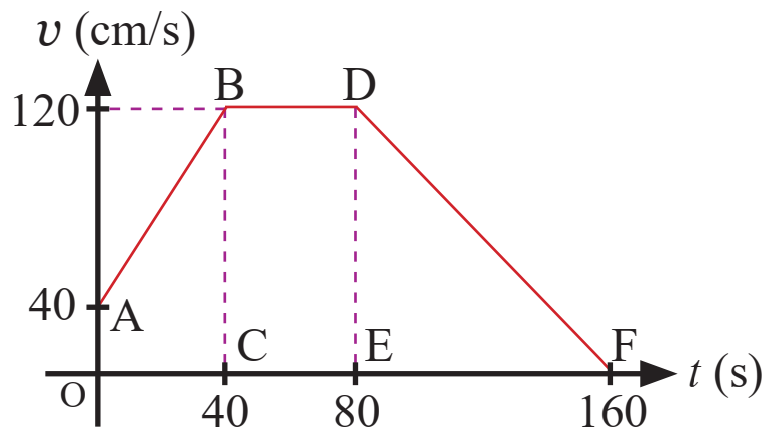
\includegraphics[width=0.4\linewidth]{../figs/BAI7-1}
			\end{center}
		}\\
		a) Từ $\SI{0}{\second}$ đến $\SI{40}{\second}$ & b) Từ $\SI{80}{\second}$ đến $\SI{160}{\second}$\\
		\dotfill & \dotfill \\
		\dotfill & \dotfill \\
		\dotfill & \dotfill \\
		\dotfill & \dotfill \\
		\dotfill & \dotfill \\
		\hline
	\end{longtable}
\end{center}
\newpage
\textbf{Phiếu số 3:} Rút ra được công thức độ dịch chuyển trong chuyển động thẳng biến đổi đều.
\begin{center}
	\begin{longtable}{|L{8.5cm}L{8.5cm}|}
		\hline
		\multicolumn{2}{|M{17cm}|}{\textbf{PHIẾU HỌC TẬP SỐ 3 \textit{(NHÓM LỚN)}	RÚT RA ĐƯỢC CÔNG THỨC\newline ĐỘ DỊCH CHUYỂN TRONG CHUYỂN ĐỘNG THẲNG BIẾN ĐỔI ĐỀU
		}}\\
		\hline
		Lớp: \dotfill & Nhóm: \dotfill\\
		\multicolumn{2}{|L{17cm}|}{Tên: \dotfill}\\
		\hline
		\multicolumn{2}{|L{17cm}|}{\textbf{Nhiệm vụ:} Dựa vào đồ thị $\left(v-t\right)$ của vật chuyển động thẳng biến đổi đều, hãy rút ra công thức xác định độ dịch chuyển theo $v_0$ , $a$, $t$.
			\begin{center}
				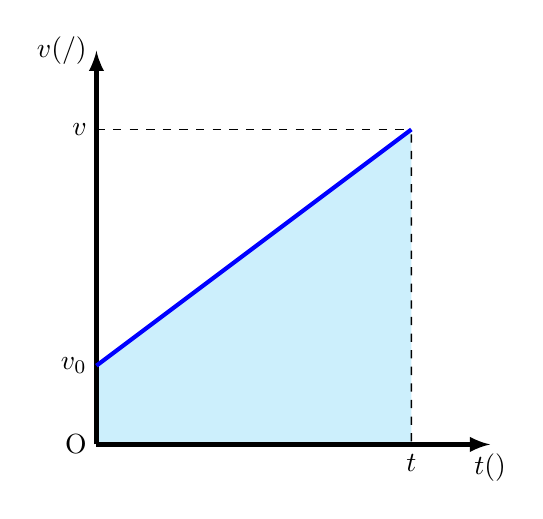
\begin{tikzpicture}  
					\coordinate (O) at(0,0);
					\coordinate (x) at(5,0);
					\coordinate (y) at(0,5);
					\coordinate (v0) at(0,1);
					\coordinate (v1) at(0,1.75);
					\coordinate (v2) at(0,4);
					\coordinate (B) at(4,4);
					\coordinate (A) at(1,1.75);
					\coordinate (C) at(4,0);
					\coordinate (D) at(1,0);
					\fill[cyan, opacity=0.2] (v0)--(B)--(C)--(O)--(v0);
					\draw[line width=0.5pt,black, dashed] (v0)--(B)--(C)--(O)--(v0);
					\draw[line width=0.5pt, dashed] (v2)--(B);
					\draw[-latex, line width=1.5pt] (O)--(x);
					\draw[-latex, line width=1.5pt] (O)--(y);
					\draw[blue, line width=1.5pt] (v0)--(B);
					\node[below] at(x) {$\xsi{t}{\left(\second\right)}$};
					\node[left] at(y) {$\xsi{v}{(\meter/\second)}$};
					\node[left] at(v0) {$v_0$};
					\node[left] at(0,4) {$v$};
					\node[left] at(O) {O};
					\node[below] at (C) {$t$};
				\end{tikzpicture}
			\end{center}
		}\\
		\multicolumn{2}{|L{17cm}|}{\dotfill}\\
		\multicolumn{2}{|L{17cm}|}{\dotfill}\\
		\multicolumn{2}{|L{17cm}|}{\dotfill}\\
		\multicolumn{2}{|L{17cm}|}{\dotfill}\\
		\hline
	\end{longtable}
\end{center}